\documentclass{emulateapj}
\submitted{{\it Submitted for publication in ApJ Letters}}
\usepackage{multirow,color,wrapfig,ulem}
\usepackage {graphicx}
%\bibliographystyle{apj}
\usepackage{graphics}
\usepackage[dvips]{epsfig}

\newcommand{\kms}{\,km~s$^{-1}$}
\def\squig{\sim\!\!}
\newcommand{\LCDM}{$\Lambda$CDM~}
\newcommand{\beq}{\begin{eqnarray}}  
\newcommand{\eeq}{\end{eqnarray}}  
\newcommand{\zz}{$z\sim 3$} 
\newcommand{\avg}[1]{\langle{#1}\rangle}  
\newcommand{\ly}{{\ifmmode{{\rm Ly}\alpha}\else{Ly$\alpha$}\fi}}
\newcommand{\hMpc}{{\ifmmode{h^{-1}{\rm Mpc}}\else{$h^{-1}$Mpc }\fi}}  
\newcommand{\hGpc}{{\ifmmode{h^{-1}{\rm Gpc}}\else{$h^{-1}$Gpc }\fi}}  
\newcommand{\hmpc}{{\ifmmode{h^{-1}{\rm Mpc}}\else{$h^{-1}$Mpc }\fi}}  
\newcommand{\hkpc}{{\ifmmode{h^{-1}{\rm kpc}}\else{$h^{-1}$kpc }\fi}}  
\newcommand{\hMsun}{{\ifmmode{h^{-1}{\rm {M_{\odot}}}}\else{$h^{-1}{\rm{M_{\odot}}}$}\fi}}  
\newcommand{\hmsun}{{\ifmmode{h^{-1}{\rm {M_{\odot}}}}\else{$h^{-1}{\rm{M_{\odot}}}$}\fi}}  
\newcommand{\Msun}{{\ifmmode{{\rm {M_{\odot}}}}\else{${\rm{M_{\odot}}}$}\fi}}  
\newcommand{\msun}{{\ifmmode{{\rm {M_{\odot}}}}\else{${\rm{M_{\odot}}}$}\fi}}  
\newcommand{\lya}{{Lyman$\alpha$~}}
\newcommand{\clara}{{\texttt{CLARA}}~}
\newcommand{\rand}{{\ifmmode{{\mathcal{R}}}\else{${\mathcal{R}}$ }\fi}}  
\newcommand{\Lsun}{\mbox{\,$L_{\odot}$}}
\newcommand{\like}{\mathscr{L}}
\newcommand{\bftheta}{\mathbf{\Theta}}
\newcommand{\degree}{\ensuremath{^\circ}}
\def\spose#1{\hbox to 0pt{#1\hss}}
\def\simlt{\mathrel{\spose{\lower 3pt\hbox{$\mathchar"218$}}
     \raise 2.0pt\hbox{$\mathchar"13C$}}}
\def\simgt{\mathrel{\spose{\lower 3pt\hbox{$\mathchar"218$}}
     \raise 2.0pt\hbox{$\mathchar"13E$}}}
\font\smcap=cmcsc10


\shorttitle{Local Group Kinematics}
\shortauthors{Forero-Romero et al.}

\begin{document}
\title{The kinematics of the Local Group in a cosmological context}
\author{
J. E.\ Forero-Romero\altaffilmark{1}, 
Y. Hoffman\altaffilmark{2}, 
S. Bustamante\altaffilmark{3}, 
S. Gottl\"ober\altaffilmark{4}, 
G. Yepes\altaffilmark{5}
}

\altaffiltext{1}{Departamento de F\'{i}sica, Universidad de los Andes, Cra. 1 No. 18A-10, Edificio Ip, Bogot\'a, Colombia, \email{je.forero@uniandes.edu.co}}
\altaffiltext{2}{Racah Institute of Physics, The Hebrew University of Jerusalem, 91904 Jerusalem, Israel}
\altaffiltext{3}{Instituto de F\'{\i}sica - FCEN, Universidad de Antioquia, Calle 67 No. 53-108, Medell\'{\i}n, Colombia}
\altaffiltext{4}{Leibniz-Institut f\"ur Astrophysik, Potsdam, An der Sternwarte 16, 14482 Potsdam, Germany}
\altaffiltext{5}{Grupo de Astrof\'{\i}sica, Departamento de F\'{\i}sica Te\'orica, Universidad Aut\'onoma de Madrid,
Cantoblanco E-280049, Spain}

\date{\today}

\begin{abstract}
   
Recent observations constrained the tangential velocity of M31 with respect to the Milky Way (MW) to be $v_{\rm M31,tan}<34.4$ \kms and the radial velocity to be in the range $v_{\rm M31,rad}=-109\pm 4.4$\kms \citep{vanderMarel12}. In this study we use a large volume high resolution N-body cosmological simulation to statistically study this kinematics in the context of the $\Lambda$CDM cosmology. We define the Local Group (LG) to be composed by two dominant separate halos hosting the MW and the M31 galaxy fulfilling certain isolation criteria. We find that the most probable values for the tangential and radial velocities in these pairs are $v_{\rm rad, \Lambda CDM}=-60\pm 15$\kms and $v_{\rm tan, \Lambda CDM}=50\pm 5$\kms. Within a similar absolute uncertainty defined by observations the pairs centered around these values are $\sim3$ times more abundant than the pairs in the observational interval. Furthermore, we find that only $\sim12\%$ of the pairs show a ratio between its tangential and radial velocity consistent with observations. This tension increases if we make a narrower selection in the pair sample to match the observational constraints on pair separation and total mass. Expressing these results in terms of the angular momentum and mechanical energy per unit mass also reflects this disagreement albeit in a less strong fashion due to the larger uncertainties inferred for these physical quantities. From these quantities Peeble's spin parameter is evaluated and is used to characterize the LG with repect to other halo pairs in $\Lambda$CDM. We also include in our analysis results from constrained simulations. The characterisation results of this study suggest that the formation and evolution of the LG differ from the average $\Lambda$CDM halo pair.
\end{abstract}

\begin{keywords}
{galaxies: kinematics and dynamics, Local Group, methods:numerical}
\end{keywords}

\section{Introduction}

The Milky Way (MW) and Andromeda galaxy (M31) are the dominant galaxies in the Local Group (LG). Astronomical observations of their mass distribution impose constraints on the standard cosmological model. The satellite overabundance problem \citep{Klypin99,Moore99}, tidal disruption features \citep{pandas09} and the disk dominated morphology \citep{Kazantzidis2008} are examples on of how LG studies are linked to the cosmological context. Detailed studies on the Magellanic Clouds dynamics and their possible link to M31 add to the interest of understanding the details of the LG kinematics and dynamics \citep{Besla2007,Tollerud2011,Knebe2011,Fouquet2012,Teyssier2012}. However, a general concern in the use of the LG as a tool for near-field cosmology \citep{Freeman2002,Peebles2010} is how typical is the LG regarding the properties of interest \citep{Busha2011,Liu2011,ForeroRomero2011,Purcell2012}. 

A new valuable piece of information in this issue is the recent observational determination of the proper-motion measurements of M31, which until recently had been out of reach \citep{vanderMarel12}. This measurement opens up the possibility to study in detail the dynamics of the LG in a cosmological context. The reported measurements set an upper bound for the tangential velocity of M31 with respect to the MW of $v_{\rm tan,M31}\leq 34.4$ km s$^{-1}$. Together with the values of the relative radial velocity of $v_{\rm rad,M31}=-109\pm 4.4$ \kms observations show that the relative motion of the MW and Andromeda is consistent with a head-on collision. With this information it is possible to ask how common is this kinematic configuration in a $\Lambda$CDM Universe.

This Letter presents such study. We use a large volume, high resolution dark matter only N-body simulation in the concordance $\Lambda$CDM cosmology to find a set of halo pairs with similar isolation criteria as inferred in the LG. We quantify these results in terms of the number of pairs with given radial and tangential velocities in the galactocentric rest frame. We also find the pairs that are consistent with a head on collision in terms of the ratio of the radial to tangential velocity $f_{\rm t}\equiv v_{\rm tan}/v_{\rm rad}<0.3$ and present these results in terms of the reduced angular momentum and mechanical energy.

In addition we make use of three N-body simulations with constrained initial conditions which are constructed to reproduce the observed large scale structure of the Local Universe on scales of a few tens of Mpc. The special feature of these simulations is that each volume features a pair of halos with the right isolation and relative positioning characteristics to be considered Local Group halos.  Finally, we provide an interpretation of these results in terms of the large scale structure environment. We find what places in the cosmic web favor the presence of dark matter halos with kinematics similar to the LG.

This Letter is structured as follows. In the next section we present the N-body simulations, the criteria we use to select LG-like halo pairs and the method we use to characterize the cosmic web. In Section \ref{sec:results} we present the results for the dynamics in these pairs in terms of the tangential/radial velocities and the orbital angular momentum/mechanical energy. In the same section we investigate what kind of large scale environment can foster the production of pairs with dynamics similar to those observed in the LG. Finally, in the last section we comment and conclude about the implications of these results in the context of the $\Lambda$CDM model.





\label{subsec:lg-sample}
\begin{figure*}
\begin{center}
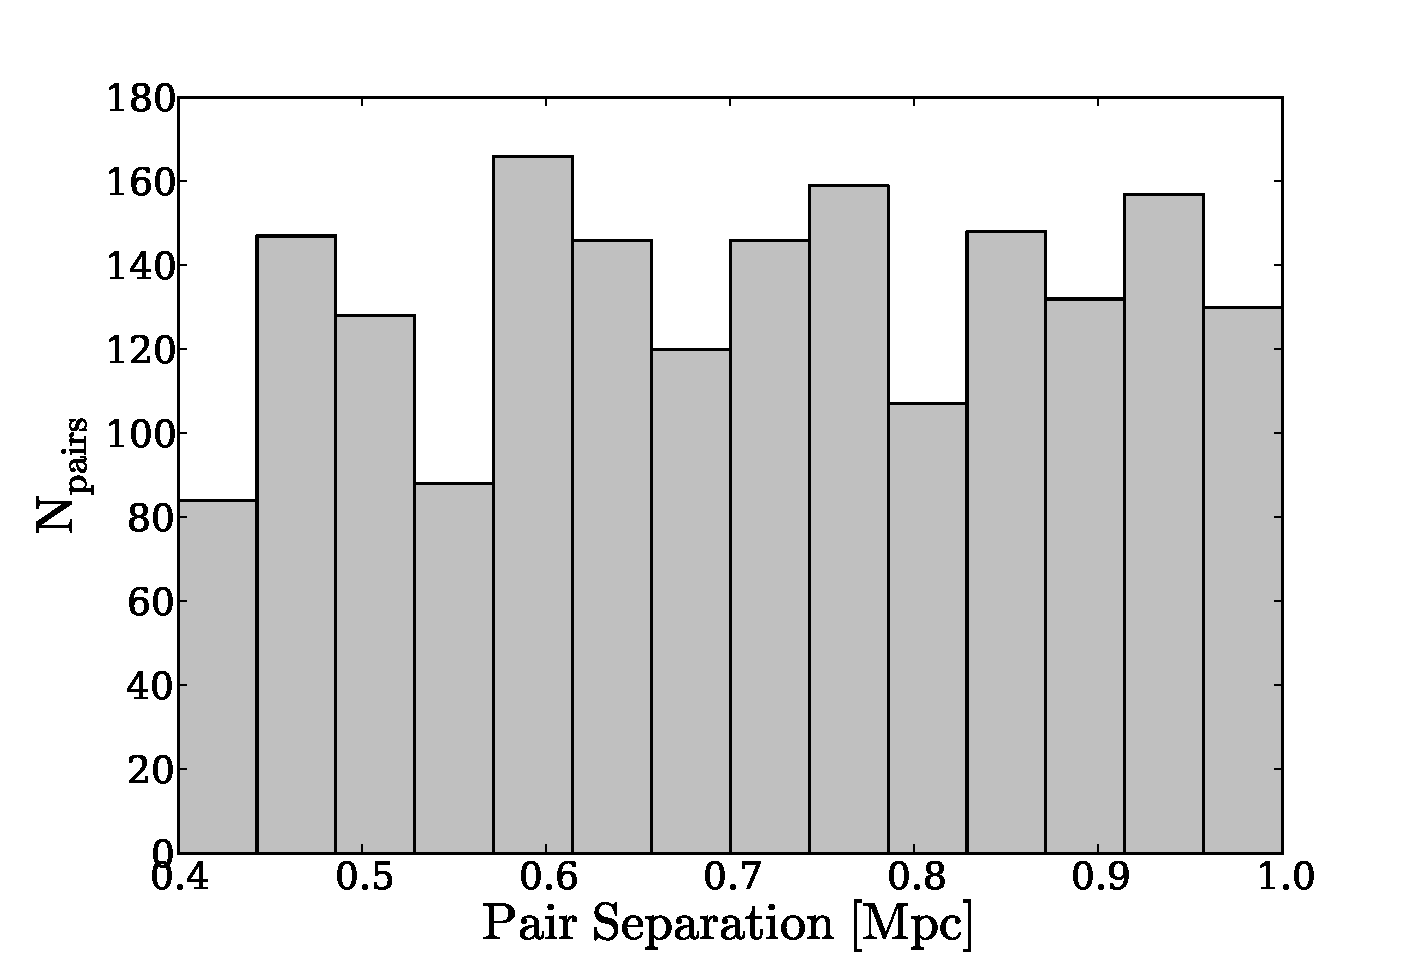
\includegraphics[keepaspectratio=true,width=0.45\textwidth]{./figures/separation_BDM.pdf}
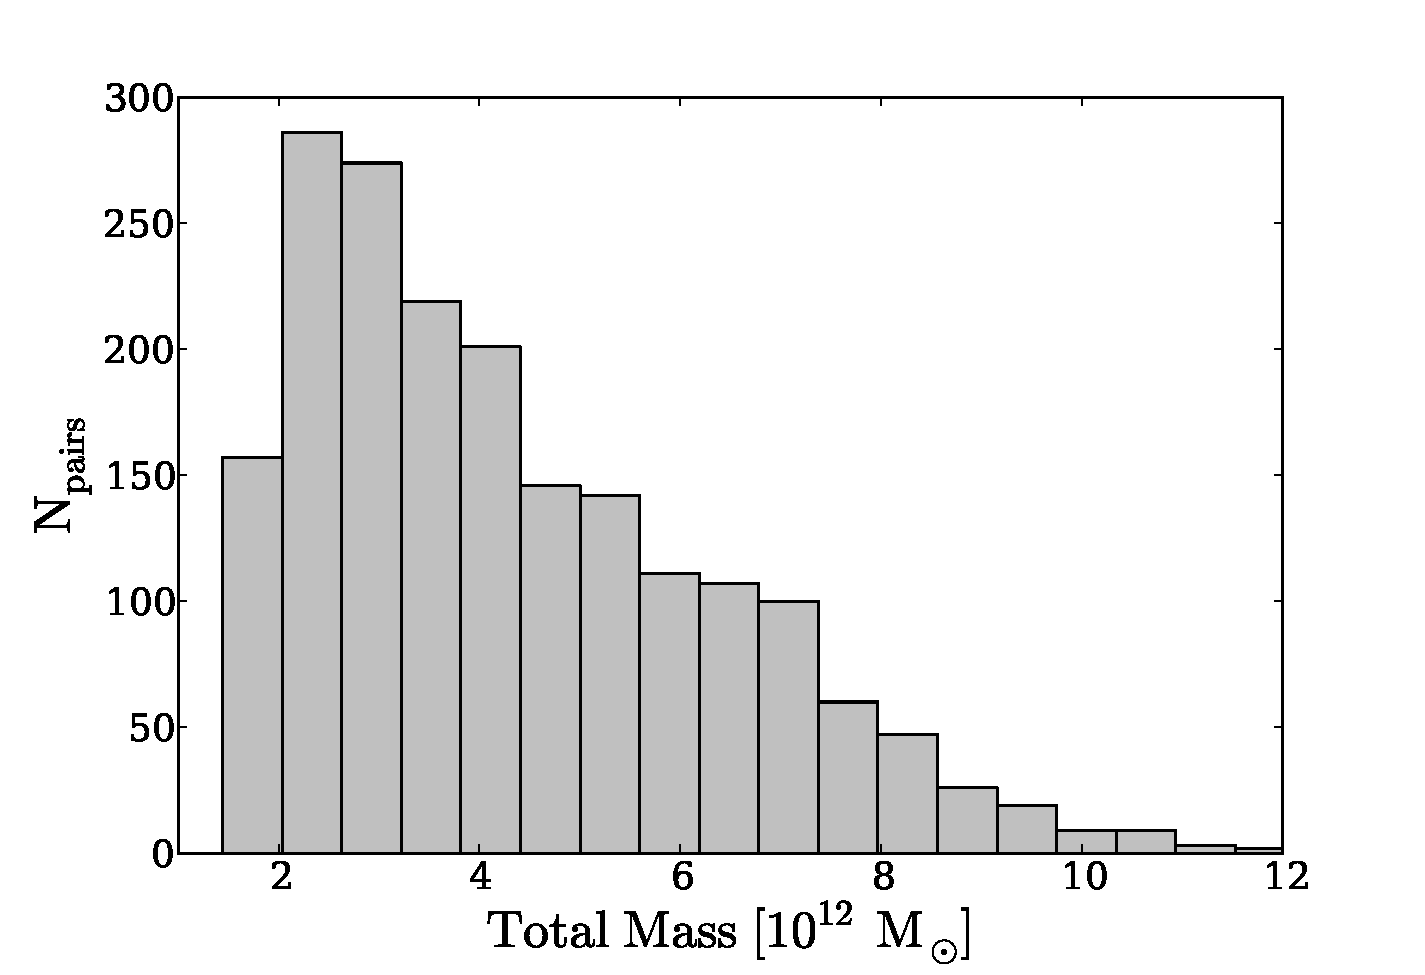
\includegraphics[keepaspectratio=true,width=0.45\textwidth]{./figures/total_mass_BDM.pdf}
\caption{\label{fig:distros} Distributions of separations and total halo mass (Milky Way and M31) in the LG-like pairs selected from the Bolshoi Simulation.}
\end{center}
\end{figure*}

\section{Simulation and Environment}
\label{sec:methods}
\subsection{The Bolshoi and Constrained Simulations}



The Bolshoi simulation follows the non-linear evolution of the dark matter density field using N-body techniques. The simulation has a cubic volume of $250$\hMpc comoving on a side, sampled with $2048^{3}$ particles. The cosmological parameters used in the simulation are $\Omega_{m}=0.27, \Omega_{\Lambda}=0.73, \sigma_{8}=0.82, h=0.70$ and $n=0.95$, corresponding to the matter density, vacuum energy density, the normalization of the power spectrum, the dimensionless Hubble constant and the index of the slope in the initial power spectrum. This set of parameters is compatible with the analysis  of the seventh year of data from the Wilkinson Microwave Anisotropy Probe (WMAP) \citep{Jarosik2011}. A detailed description of this simulation can be found in \citep{Bolshoi}.

With these parameters the mass per particle is $m_{p}=1.4\times 10^{8}$\hMsun. In this paper we use algorithms obtained through the Bound Density Maxima (BDM) algorithm \citep{KlypinBDM}. The halos are selected to have an overdensity of 200 times the critical density. Furthermore, we only include in the analysis haloes whose center is located outside the virial radius of any other halo.  We have obtained the data through the public available Multidark database \footnote{{\tt http://www.multidark.org/MultiDark/}} \citep{2011arXiv1109.0003R}. The database allows us to obtain the comoving positions, peculiar velocities and masses for all the halos in the simulation volume at $z=0$. The positions and velocities of these haloes correspond to the average values of the $250$ most bound particles. The Hubble flow is taken into account to convert the peculiar velocities into physical velocities and allow for a comparison with observations. We have verified that the main conclusions of this paper hold in the case of halos defined by a FOF algorithm with a linking lentgth 0.17 times the interparticle distance.

The constrained simulations we use in this Letter are part of the Constrained Local UniversE Simulations (CLUES) project whose main objective is to reproduce the large scale structure in the Local Universe as accurately as possible. The algorithm and observational constraints to construct the initial conditions are  described in \citep{clues2010}.  We use three dark matter only simulations, each has a cubic volume of $64$\hMpc on a side, with the density field sampled with $1024^3$ particles. The cosmological density parameter is $\Omega_m=0.28$, the cosmological constant $\Omega_{\Lambda}=0.72$, the dimensionless Hubble parameter $h=0.73$, the spectral index of the primordial density perturbations $n=0.96$ and the power spectrum normalization $\sigma_{8}=0.817$, also consistent with WMAP 7th year data. 


\subsection{The LG-sample}
Based on the BDM catalogs in the Bolshoi simulation we construct a halo pair sample with masses and isolation properties consistent with the inferred properties for the MW and M31. The characteristics we impose to define a LG-like halo pair are the following:

\begin{enumerate}
\item Each halo has a mass in the range $5\times10^{11}\hMsun <M_{h}<5\times 10^{12}\hMsun$.
\item With respect to each halo, there cannot be any other halo within the mass range $5\times10^{11}\hMsun <M_{h}<5\times 10^{12}\hMsun$ closer than its partner. It means that there cannot be ambiguity on the identity of the pair members.
\item The relative radial velocity between the two halos is negative \citep{vanderMarel12}.
\item The distance between the center of mass of the halos must be less than $0.7$\hMpc \citep{ribas05,vanderMarel08}.
\item There cannot be halos more massive than $5\times 10^{12}$\hMsun within a radius of $2$\hMpc with respect to every object centre \citep{Karachentsev04,Anton09}.
\item There cannot be halos more massive than $5\times 10^{13}$\hMsun within  a radius of $3$\hMpc with respect to every object centre \citep{Karachentsev04}.
\end{enumerate}

This sample in the Bolshoi simulation has $1923$ pairs. Additionally, there is a sample of three (3) pairs constructed from the three constrained realizations. These pairs fulfill all the above mentioned conditions and additionally are located in a place with the right distances with respect to the Virgo cluster in the simulation. Figure \ref{fig:distros} show the  distribution of separations and total pair mass computed from the $1923$ pairs in the Bolshoi simulation. 

Additional constraints will be set on this population in order to match the observational estimates for separation and total mass. The full observational characteristics that we take in this Letter for the MW-M31 pair are listed in Table \ref{table:1}. We refer to this sample as a reduced LG-like sample. The additional characteritiscs we impose in addition to the ones listed above are

\begin{enumerate}
\item The separation betwen the center of mass of the halos is in the range $700-800$kpc \citep{ribas05,vanderMarel08}.
\item The total mass of the two halos is in the range $1-4\times 10^{12}$\Msun \citep{vanderMarel12}.
\end{enumerate}



\begin{table}
\caption{Summary of the kinematic properties for M31 in the galactocentric frame as reported by \citep{vanderMarel12}. Values in parenthesis correspond to vector components. $\sigma_{\bf x}$ represents the uncertainty on the components of vector ${\bf x}$}
\begin{center}
\begin{tabular}{ccc}\hline\hline
${\bf r}_{\rm M31}$ & (kpc) &$(-378.9, 612.7, -283.1)$\\
$\sigma_{{\bf r}, {\rm M31}}$ & (kpc) &$(-18.9, 30.6, 14.5)$\\
${\bf v}_{\rm M31}$ & (\kms) & $(66.1, -76.3, 45.1)$\\
$\sigma_{{\bf v},{\rm M31}}$ & (\kms) &$(26.7, 19.0, 26.5)$\\
$v_{\rm M31,rad}$ &(\kms) & $-109.3\pm 4.4$\\
$v_{\rm M31,tan}$ &(\kms) & $<34.4$\\
$r_{\rm M31}$ &(kpc) & $770\pm 40$\\
$M_{\rm 200,MW} + M_{\rm 200, M31}$ & ($10^{12}\Msun$) & $3.14\pm 0.58$\\\hline
\end{tabular}\\
\vspace{1mm}
Note: the observational uncertainties in the position vector correspond to a $5\%$ in each component consistent with the uncertainties in the distance \citep[see references in][]{vanderMarel08}
\end{center}
\label{table:1}
\end{table}



\section{Results}
\label{sec:results}




\subsection{Radial and tangential velocities}

Figure \ref{fig:rt} summarizes the central finding of this Letter. Most of the LG-like pairs (left panel) in the Bolshoi Simulation and the pairs in the constrained simulation have radial and tangential velocities notably different from the observational constraints.  The most probable velocities in the simulation are around $v_{\rm rad,\Lambda CDM} = -70\pm5$\kms and $v_{\rm tan,\Lambda CDM} = 50\pm5$ \kms, where the uncertainties in these values reflect the minimum grid size needed to obtain robust statistics from the 2D histogram. There are $23$ pairs in the region centered around those values within an interval width comparable with the uncertainties in the observational constraints ($\sigma_{\rm tan}=17$\kms and $\sigma_{\rm rad}=4$\kms.) In contrast, there are only $8$ pairs in the interval allowed by observations. This makes the LG-like pairs consistent with observations $\sim3$ times less likely to be found than a pair with velocities around $v_{\rm rad,\Lambda CDM}-v_{\rm tan,\Lambda CDM}$.

From Figure \ref{fig:rt} it is also clear that there is a significant number of pairs with a high tangential-to-radial velocity ratio. The peak in the pair number density is located around a region of $f_{\rm t}\equiv v_{\rm tan \Lambda CDM}/v_{\rm rad \Lambda CDM}\sim 0.7$, while the observations suggest $f_{\rm t}<0.32$. In the Bolshoi Simulation, out of $1923$ LG-like pairs we find that $242$ pairs ($\sim 12\%$ of the total sample) have values for $f_{\rm t}$ consistent with that constraint. The three pairs from the constrained realizations are also outside the region of the most probable values in a $\Lambda$CDM cosmology with tangential-to-radial ratios of $f_{\rm t}= 0.35, 0.45, 0.73$.

The right panel in Figure \ref{fig:rt} shows the results of making narrower selection of the LG-like pairs to separations between $700-800$ kpc and a total mass in the two halos to be in the range $1-4 \times 10^{12}$\Msun. This change emphasizes the tension found from the full LG-like sample. The sample is smaller ($1923$ pairs are reduced to $158$) and the values corresponding to the highest density region in the radial-tangential velocity plane are  $v_{\rm rad,\Lambda CDM} = -50\pm5$\kms and $v_{\rm tan,\Lambda CDM} = 50\pm5$\kms with $5$ pairs around that value and zero pairs consistent with observations. This shows that the atypical LG dynamics in $\Lambda$CDM and the low fraction of radially dominated velocities are robust results with respect to the separation and total mass conditions used to define the LG-like pairs.  We note that this tighter selection also excludes 2 of the 3 pairs from the constrained simulations. Taking into account the results for the two different kinds of samples, we find that that the prefered values for the tangential and radial velocity components of halo pairs are bound by the values  $v_{\rm rad,\Lambda CDM} = -60\pm 15$\kms and $v_{\rm tan,\Lambda CDM} = 50\pm5$ \kms. 



\begin{figure*}
\begin{center}
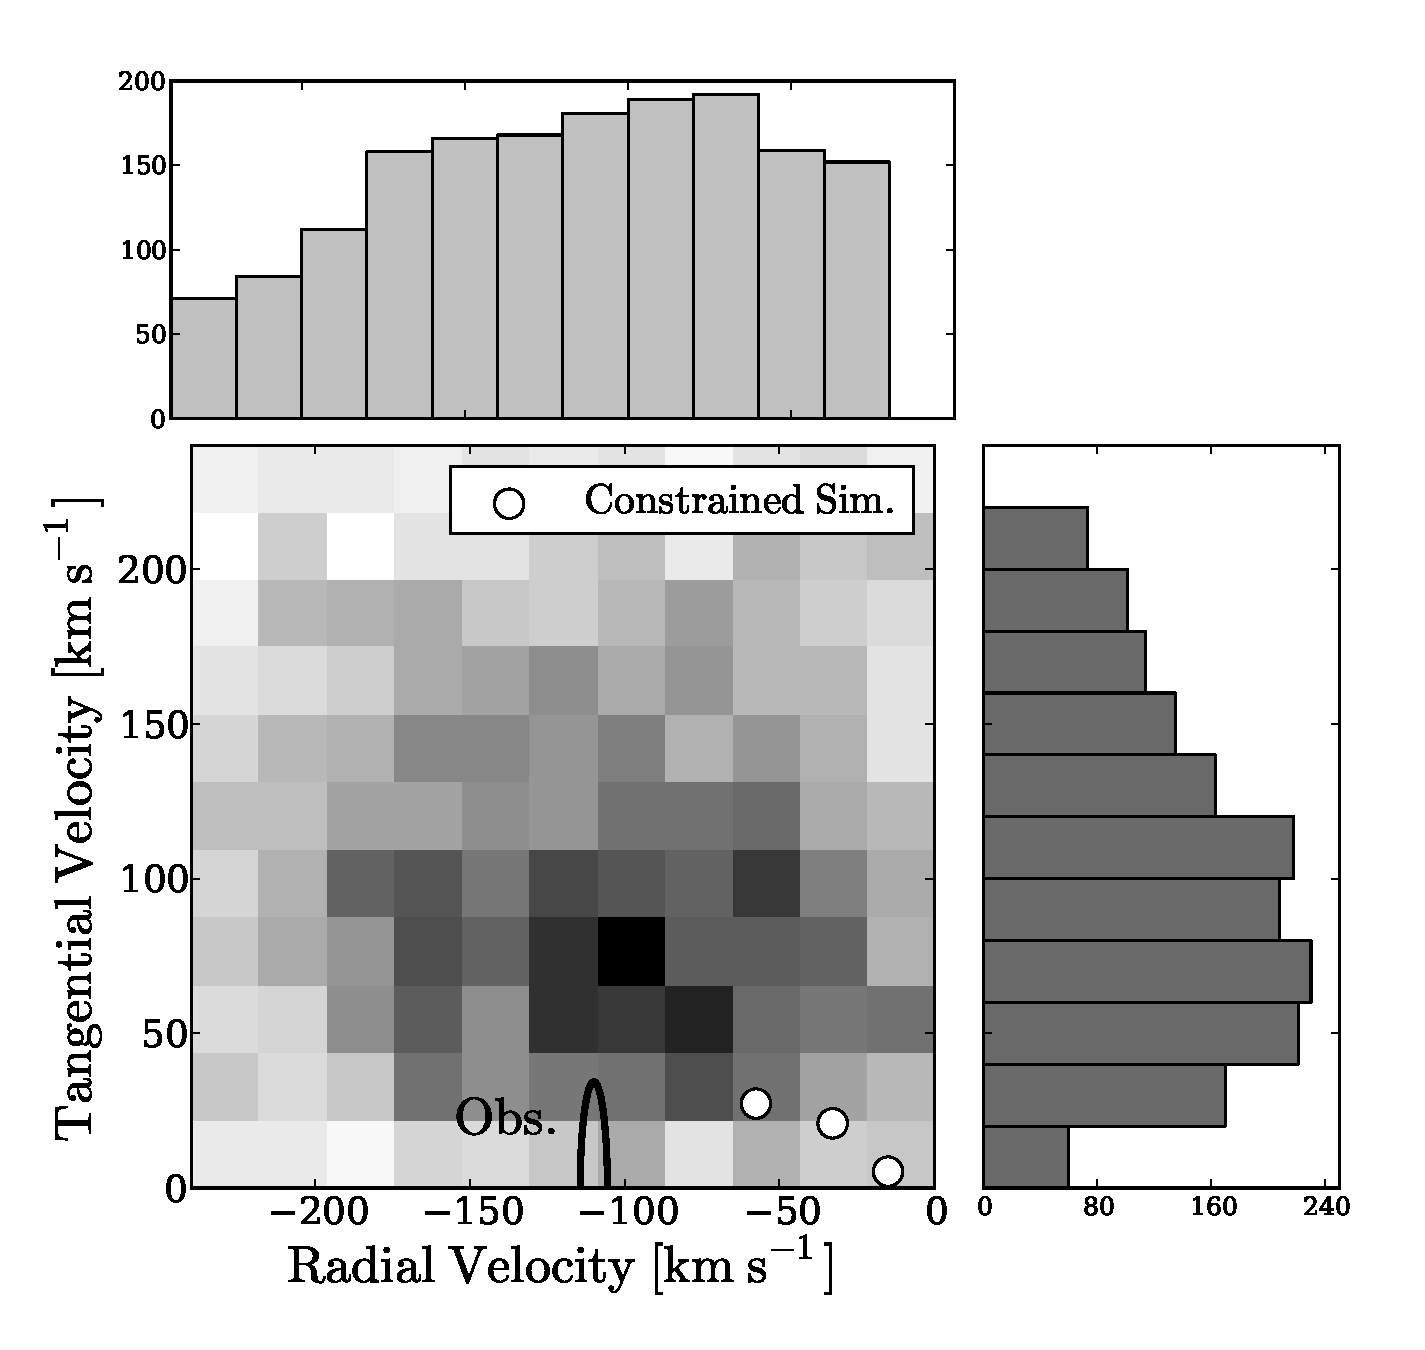
\includegraphics[keepaspectratio=true,width=0.46\textwidth]{./figures/test_rt_BDM.pdf}
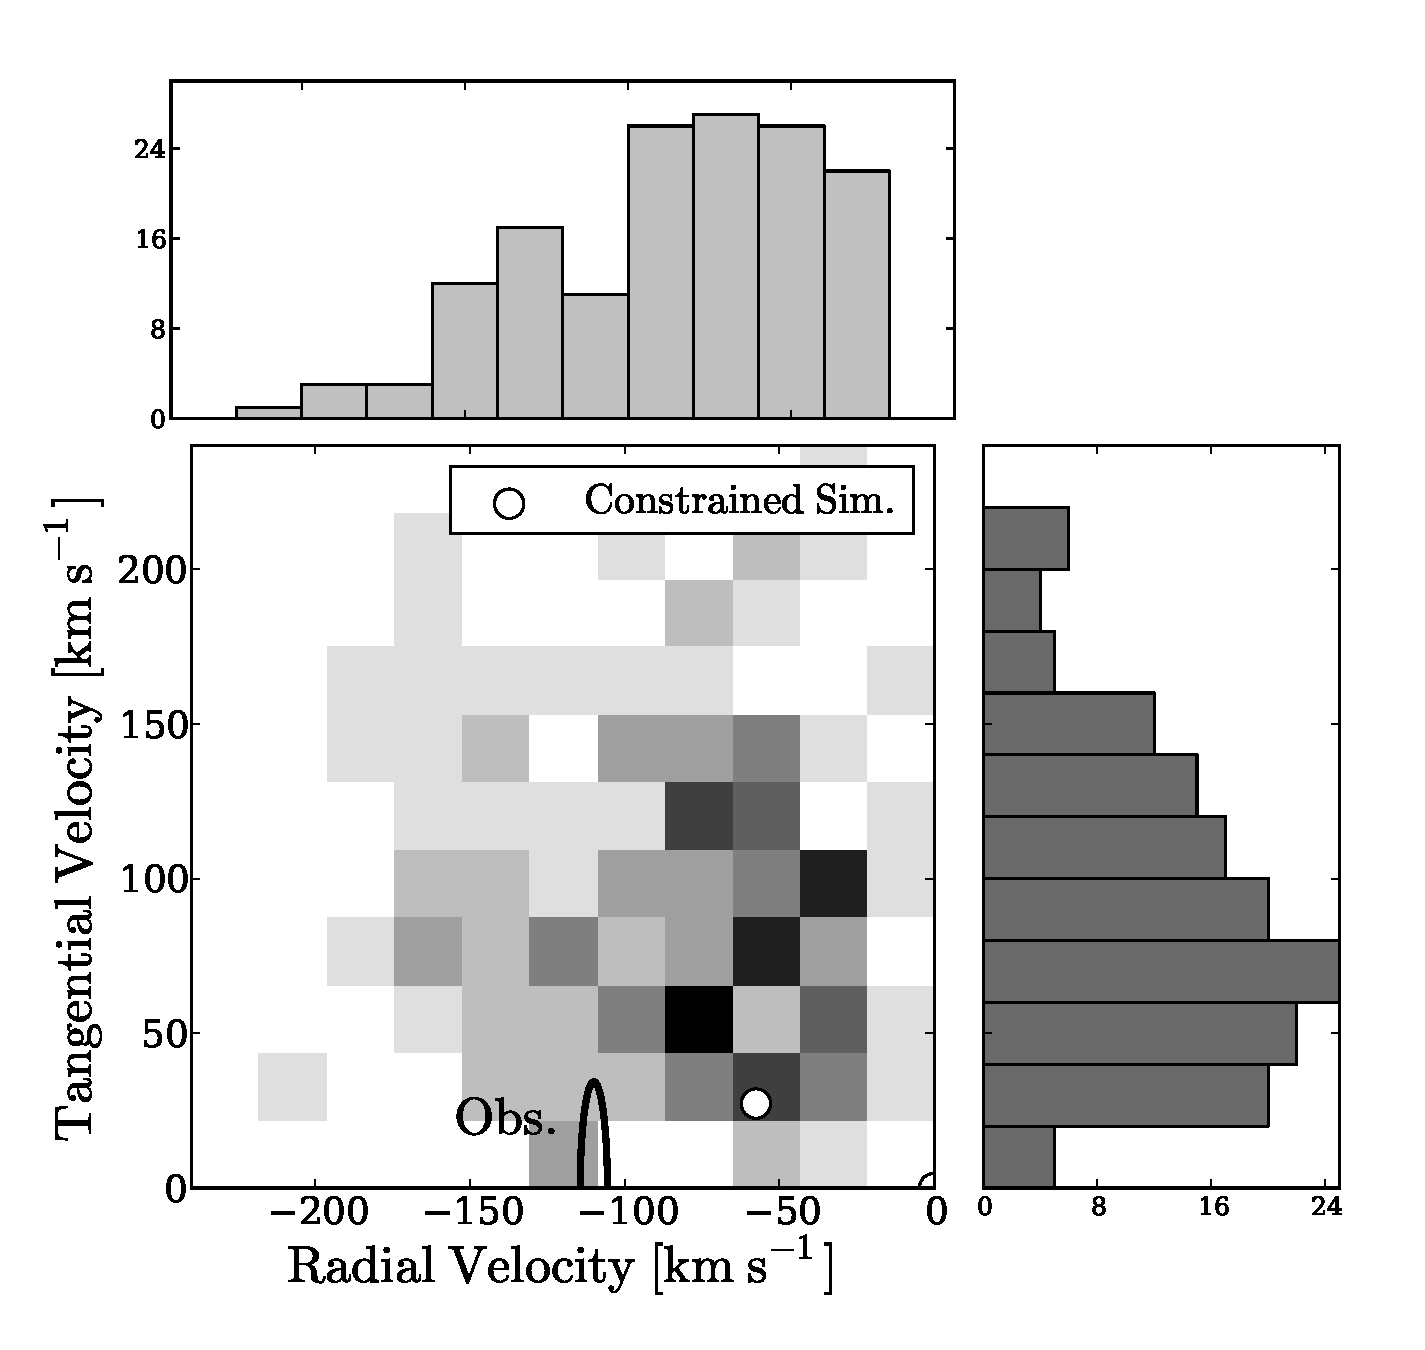
\includegraphics[keepaspectratio=true,width=0.46\textwidth]{./figures/test_rt_BDM_narrow.pdf}
\caption{Histograms of the radial and tangential velocities for LG-like halo pairs in the Bolshoi simulation. The left panel corresponds to the general LG-like pair simple, the right panel corresponds to the subsample with cuts on pair separation and total mass, matching the observational constraints. The squared panel shows as a shaded histogram the number of pairs on the radial and tangential velocities plane. The rectangular panels show the histograms when only one of the velocity components is used to bin the data. The half ellipse corresponds to the observed observational constraints for M31 in the Galactocentric rest frame: $v_{\rm rad}=109.2\pm 4.4$ km s$^{11}$ and $v_{\rm tan}< 34.4$ km s$^{-1}$ \citep{vanderMarel12}. The circles represent the positions of the pairs from the constrained simulations. The highest number density in the left panel is obtained around $v_{\rm rad,\Lambda CDM} = -70\pm5$ \kms, $v_{\rm tan,\Lambda CDM} = 50\pm5$ \kms, for the right panel it is located around $v_{\rm rad,\Lambda CDM} = -50\pm5$ \kms, $v_{\rm tan,\Lambda CDM} = 50\pm5$ }
\label{fig:rt}
\end{center}

\end{figure*}

\subsection{Reduced Angular Momentum and Energy}

\begin{figure*}
\begin{center}
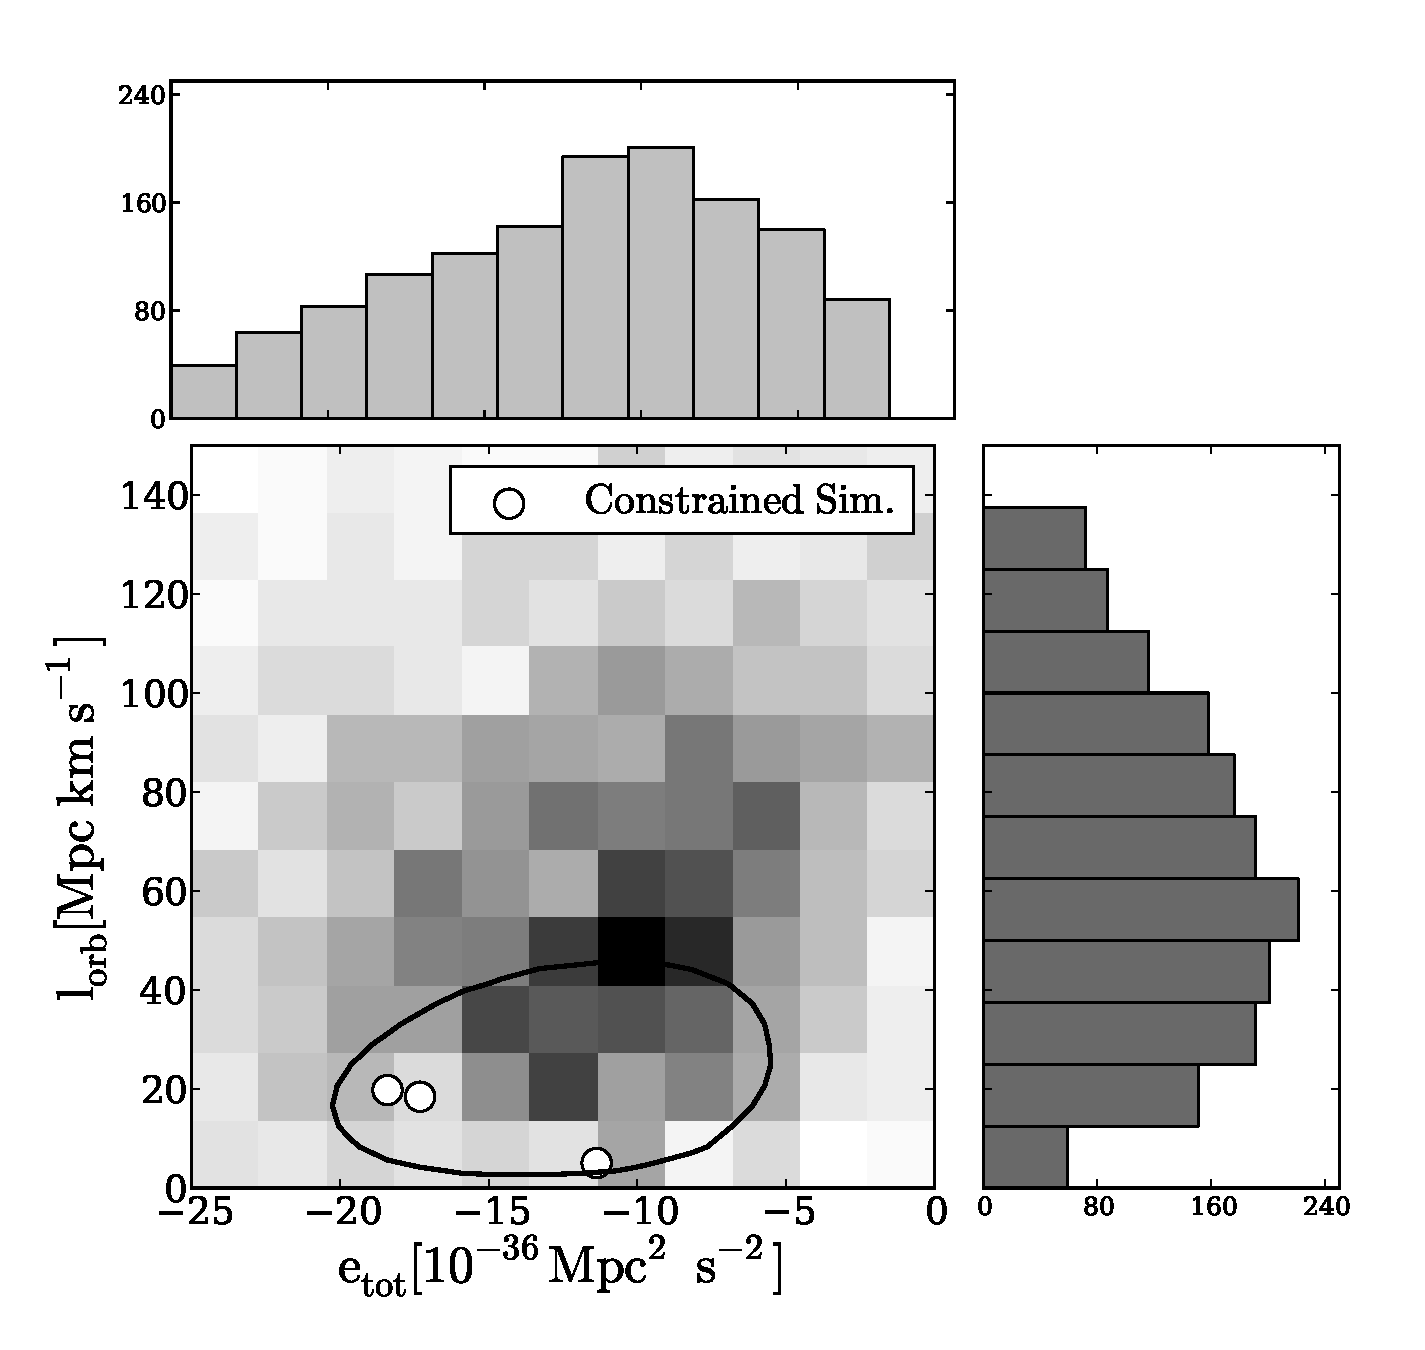
\includegraphics[keepaspectratio=true,width=0.46\textwidth]{./figures/test_EJ_BDM.pdf}
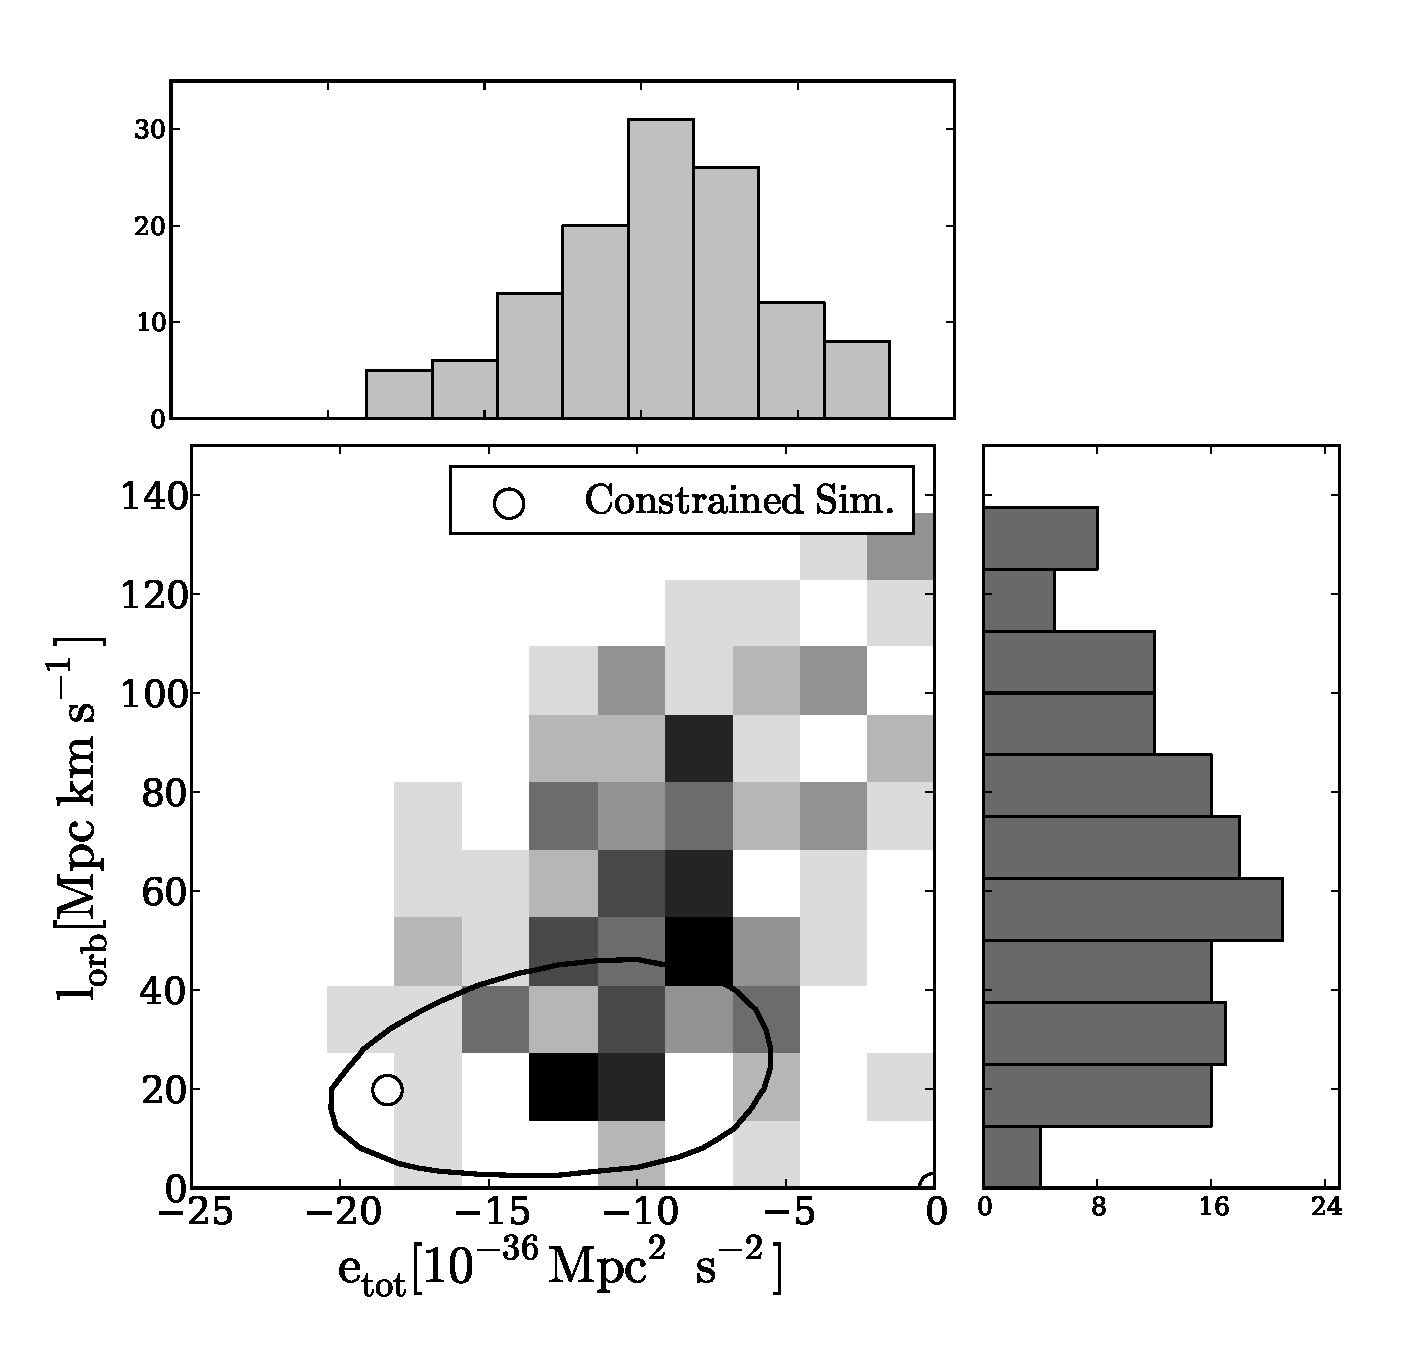
\includegraphics[keepaspectratio=true,width=0.46\textwidth]{./figures/test_EJ_BDM_narrow.pdf}
\caption{Histograms of the orbital angular momentum ($l_{\rm orb}$) and mechanical energy ($e_{\rm tot}$) per unit of reduced mass calculated considering the halos as point masses. The panel distribution is the same as in Figure \ref{fig:rt}. The contour line encloses $68\%$ of the Monte Carlo generated points to estimated the uncertainties from the observational values summarized in Table 1. The constraints in this plot are less restrictive than in Fig.\ref{fig:rt} due to added uncertainties on the tangential velocity ($100\%$), the square of the norm of the velocity ($40\%$) and the total mass of the two halos ($20\%$). }
\label{fig:EJ}
\end{center}
\end{figure*}




To gain additional physical insight we consider the two halos as points of mass $m_{\rm M31}$ and $m_{\rm MW}$. In the center of mass their orbit has an angular momentum $L=\mu|{{\bf r}_{\rm M31}}\times{\bf v}_{\rm M31}|$ and mechanical energy $E=\frac{1}{2}\mu |{\bf v}_{\rm M31}|^2 - G\mu M/|{\bf r}_{\rm M31}|$, where the total mass is $M=m_{\rm M31}+m_{\rm MW}$, the reduced mass is $\mu=m_{\rm M31}m_{\rm MW}/M$ and $G$ is the gravitational constant. We express the results of the previous section in terms of the reduced angular momentum and energy $l_{orb}=L/\mu$ and $e_{\rm tot}=E/\mu$. 

This formulation has a clear theoretical advantage if one considers the angular momentum and the mechanical energy as quasi-conserved dynamical quantities. This means that, after some formation time, these quantities do not significantly evolve as it is the case for the radial and tangential velocities. Conversely, there is an observational disadvantage. These quantities have to be derived from observations, increasing the uncertainties in their determination.

In Table \ref{table:1} we list the M31 position (${\bf r}_{\rm M31}$), M31 velocity (${\bf v}_{\rm M31}$) and total mass ($M$) that we use to estimate the uncertainties in the $e_{\rm tot}-l_{\rm orb}$ plane. To do this we generate $10^6$ pairs with different values for these three variables using a Gaussian distribution for each vector component with a variance equal to their uncertainties ${\sigma_{\bf r}}_{\rm M31}$ and ${\sigma_{\bf v}}_{\rm M31}$).. For each pair we calculate its $l_{\rm orb}$ and $e_{\rm tot}$ values.  

The results are summarized in Figure \ref{fig:EJ} following the same plotting conventions from Figure \ref{fig:rt}. The closed line is the iso-density contour in the 2D histogram enclosing $68\%$ of the Monte Carlo generated pairs consistent with observations. The poor observational constraints on the $e_{\rm tot}-l_{\rm orb}$ plane in comparison to the radial-tangential velocity plane come from the fact that we are adding up large uncertainties in three different aspects. First, the tangential velocity has a $100\%$ uncertainty, making the angular momentum compatible with very low and high values. Second, the uncertainty on the square of the norm of the velocity has an uncertainty of $40\%$, having an impact on the kinetic energy. Third, the uncertainty in the total mass of the Local Group is close to $20\%$, which has an impact on the potential energy. In Figure \ref{fig:EJ} the angular momentum does not reach a zero value at the 1-$\sigma$ as one could expect from Fig. \ref{fig:rt}, however it does reach a zero value when the isocontour encloses $80\%$ of the total number of generated points. The reason for this small difference is that our Monte Carlo simulation takes as a starting point the components of the 3D velocity. In turn, these values have uncertainties derived by MonteCarlo techniques, unlike the observational uncertainties directly inferred from the measured tangential and radial velocity components.


In the right panel of Figure \ref{fig:EJ} we see that further reduction of the LG-like pairs following the procedure decribed for the right panel of Figure \ref{fig:EJ} makes them occupy a narrower region in the total energy and orbital angular momentum plane. We also see that $e_{\rm tot}$ becomes more constrained that $l_{\rm orb}$. Under the assumption of quasi-conserved quantity a narrower region in the $e_{\rm tot}-l_{\rm orb}$ plan implies that the formation and evolution conditions for the pairs in that region must be similar. In this case the agreement with observations is moderate. A reduction by a factor of $2$ in the uncertainty of the tangential velocity showing that the tangential velocity is below $17$\kms would clearly bring the observations in the region of low $l_{\rm orb}$, clearly outside the average $\Lambda$CDM expectation.


\begin{figure*}
\begin{center}
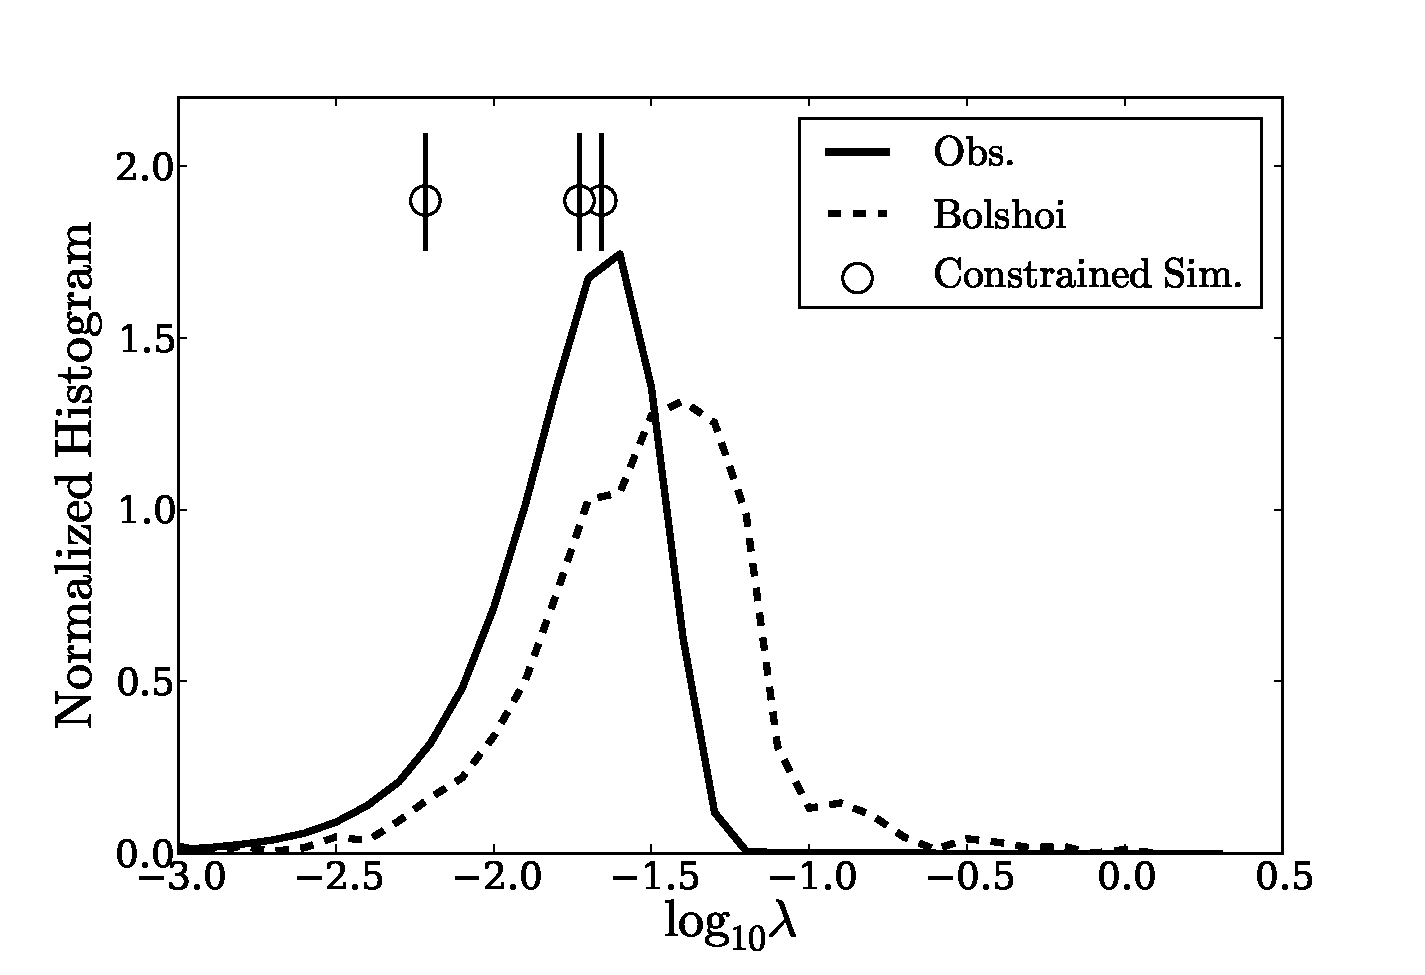
\includegraphics[keepaspectratio=true,width=0.46\textwidth]{./figures/test_lambda_BDM.pdf}
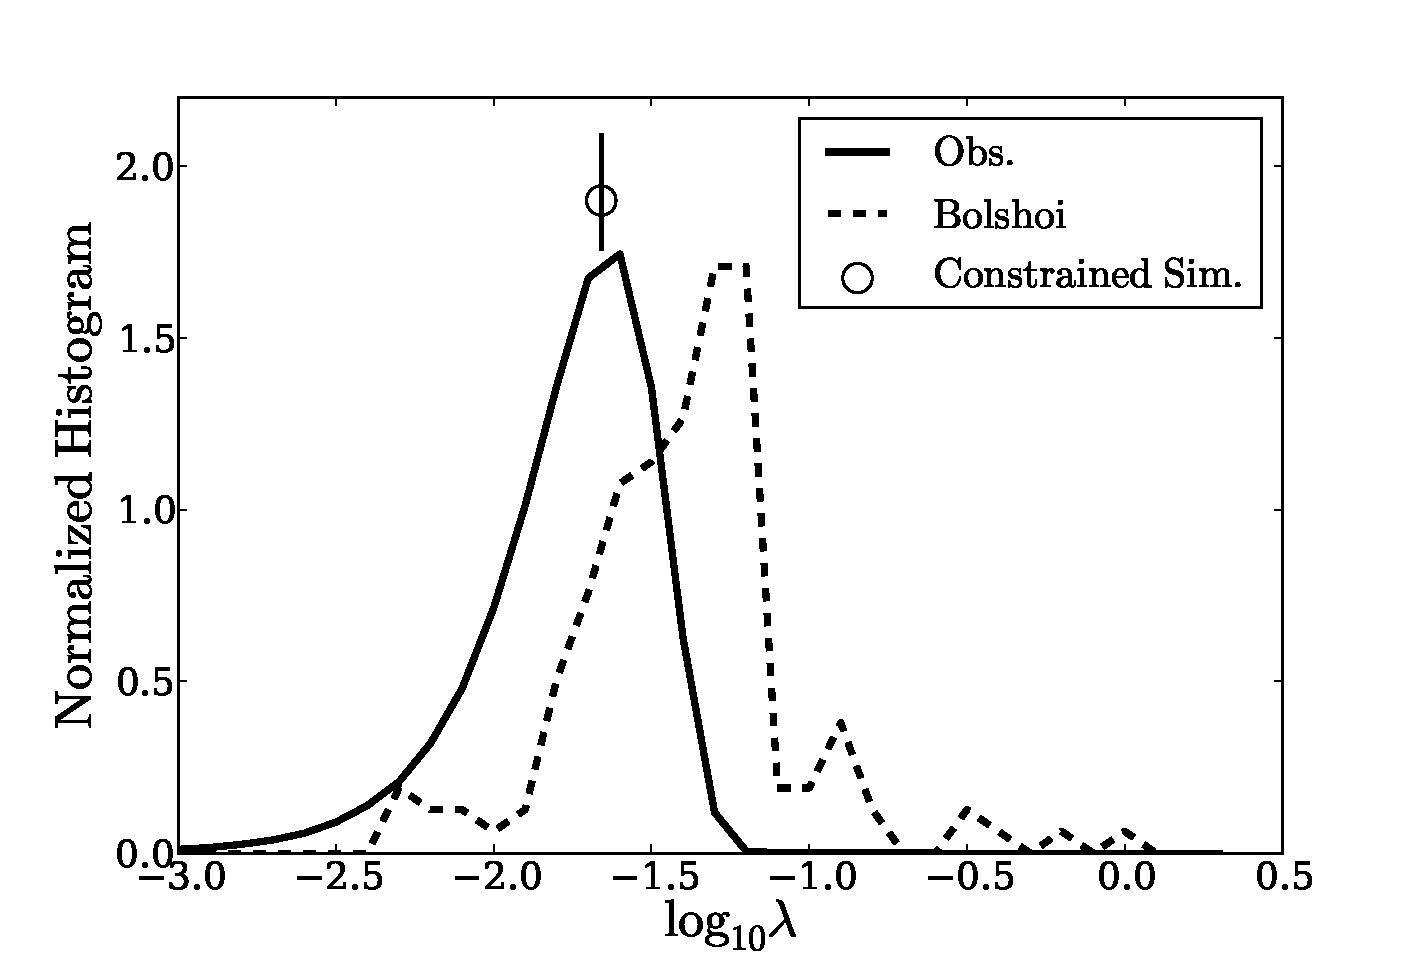
\includegraphics[keepaspectratio=true,width=0.46\textwidth]{./figures/test_lambda_BDM_narrow.pdf}
\caption{{\rm \label{fig:lambda} Normalized histograms of Peeble's spin parameter $\lambda$ for the pairs in the Bolshoi simulation and its infered values for the LG from the observational constraints from a Monte Carlo simulation. The left panel includes all the LG-pairs while the right panel includes a reduced sample of pairs that match the separation and total mass infered from Local Group observations. The vertical lines with the white dots represent the values inferred for pairs in the constrained simulations.}}
\label{fig:lambda}
\end{center}
\end{figure*}



\subsection{Dimensionless Spin Parameter}

The imensionless spin parameter $\lambda$ \citep{Peebles1971} is used here to characterize the dynamical state of the observed and simulated LGs. The parameter measures the dynamical role of the angular momentum in terms of the gravitational attraction and is defined by

\begin{equation}
\lambda = \frac{\mu^{3/2} l_{\rm orb} \sqrt{e_{\rm tot}}}{G M^{5/2}}, 
\end{equation}

where the $\mu=m_{\rm M31}m_{\rm MW}/M$ is the reduced mass for the pair.


We compare the distribution for  $\lambda$ obtained from the pair population in the Bolshoi simulation and the distribution from the MonteCrlo simulation used to estimate the uncertainties on $e_{\rm tot}$ and $l_{\rm orb}$. The results can be found in Figure \ref{fig:lambda}. The left panel shows the results from the full sample of isolated pairs while the right panel corresponds to the smaller pair sample with restrictions on the separation and total mass. Both panels in Figure \ref{fig:lambda} tell in a clearer way the story sketched in Figure \ref{fig:EJ} on the $e_{\rm tot}-l_{\rm orb}$ plane. The expected configuration in energy and angular momentum of the LG is slightly inconsistent with the expectation from halo pairs in $\Lambda CDM$. 

The spin parameter $\lambda$ seems to be lower in the observed LG than the average expectation from $\Lambda$CDM. In observations the mean of the distribution is $\log_{10}(\lambda_{\rm LG})=-1.76$, while $\log_{10}(\lambda_{\rm \Lambda CDM})=-1.51$ for the full LG-like sample and $\log_{10}(\lambda_{\rm \Lambda CDM})=-1.38$ for the reduced sample. In the case where the pairs are restricted to have the same total mass and separation as the observational constraints, the reduced energy $e_{\rm tot }$ in the simulation are is close to the range define by observations, the disagreement in $\lambda$ comes mostly from the values in the reduced orbital angular momentum $j_{\rm orb}$ which is lower in the observations than the $\Lambda$CDM expectation.

The left panel in Figure \ref{fig:lambda} shows the results from the three constrained simulations with values $\log_{10}(\lambda_{\rm CLUES})=-2.21$, $-1.72$ and $-1.65$. In this case all cases seem to be a better match to the observational expectations than to the $\Lambda$CDM pair population. In the case of tigher restrictions on the separation and total mass only one pair in the constrained simulations is retained, its $\log_{10}\lambda$ value of $1.65$ matches with the observational value $\log_{10}(\lambda_{\rm LG})=-1.76$.


\section{Conclusions}
We have presented a comparison between the observed kinematics for the M31 in the galactocentric restframe and the expectations for a large N-body cosmological simulation in the $\Lambda$CDM cosmology. In the simulation we select a sample of halo pairs in the mass range $5\times 10^{11}<M_{h}/\hMsun<5\times 10^{12}$ that closely match the isolation conditions of the Local Group from other massive structures. While the observations show that M31 moves towards us with a highly radial velocity, the simulation shows that the most common configuration at $z=0$ has values $v_{\rm rad, \Lambda CDM}=-65\pm5$\kms and $v_{\rm tan, \Lambda CDM}=62\pm5$ \kms. 


Using the same absolute values for the uncertainty in the observed velocity components, we find that halos within the preferred $\Lambda$CDM values are five times more common than pairs compatible with the observational constraint.  The qualitative nature of these results is still valid after a narrower selection on separation and total pair mass. Additionally, pairs with a fraction of tangential to radial velocity $f_{\rm t}<0.32$ (similar to observations) represent $8\%$ of the total sample of LG-like pairs. Making an tighter selection to match the observational constraints on the separation and total mass results in zero pairs compatible with observations.

Approximating the LG as two point masses we express the above mentioned results in terms of the orbital angular momentum $l_{\rm orb}$ and the mechanical energy $e_{\rm tot}$ per unit of reduced mass. We find that the uncertainties in the tangential velocity, the square of the norm of the velocity and the total mass in the LG produce poorer constraints on the number of simulated pairs that are consistent with the observations. Nevertheless, in the case of the LG-pair sample that also fulfills the separation and total mass criteria there is a slight tension between simulation and observation. A reduction by a factor of $2$ in the observational uncertainty on the radial velocity would clarify this issue.

In the three pairs from constrained simulations we find kinematics dominated by radial velocities. However their velocity components differ from the observational constraints and their mechanical energy and orbital angular momentum are in broad concordance with observations. There is only one pair that fullfills all the separation, total mass constraints and matches the most probable value for the dimensionless spin parameter $\lambda$ inferred from observations. 

The $\lambda$ spin parameter is itself a useful instrument to gauge the dynamical state of pairs. Reduced uncertainties in masses, distances and velocities can be included to produce an updated estimate for this parameter. This will immedialtly improve the statistical comparison between our Local Group and the expectations from $\Lambda$CDM.

In this Letter we have shown that LG-like pairs in $\Lambda$CDM show prefered values for their relative velocities, angular momentum and total mechanical energy. The values for the orbital angular momentum and energy, merged into the $\lambda$ spin parameter, are in mild disagreement with the observational constraints. However, there is a strong tension with the precise values for the radial and tangential velocities.

Under the approximation of consevartion of the orbital angular momentum and mechanical energy, we see that an agreement in the total angular momentum and energy and a marked difference with the precise balance between today's radial and tangential velocities could only be explained if the initial conditions for the formation of the Local Group are special in comparison to the initial conditions of any other pair of dark matter halos in the $\Lambda$CDM cosmology. 

We consider that reducing the uncertainties in the observations relevant to this study are needed. Likewise, additional theoretical work to understand the origin and implications of this result deserve further study.

\label{sec:conclusions}
\section*{Acknowledgments}  
J.E.F-R acknowledges financial support from the Vicerrector\'{\i}a de Investigaciones at Universidad de los Andes through its {\it Fondo de Apoyo a Profesores Asistentes} and the Peter and Patricia Gruber Foundation through its fellowship administered by the International Astronomical Union. J.E.F-R also acknowledges early discussions with Alejandro Garc\'ia that motivated this work.

The data and source code and instructions to replicate the results of this paper can be found as a github repository {\texttt https://github.com/forero/LG\_Kinematics/}. Thanks to the IPython community \citep{IPython}. Thanks to Jessica Kirkpatrick for releasing her Python code to make nice plots of 2D histograms. 

The MultiDark Database used in this paper and the web application providing online access to it were constructed as part of the activities of the German Astrophysical Virtual Observatory as result of a collaboration between the Leibniz-Institute for Astrophysics Potsdam (AIP) and the Spanish MultiDark Consolider Project CSD2009-00064. The Bolshoi simulation was run on the NASA's Pleiades supercomputer at the NASA Ames Research Center.


\bibliographystyle{apj}
\bibliography{references} 


\end{document}

